\documentclass[Japanese]{dicomopapers}
%\documentclass[Japanese,noauthor]{dicomopapers}

% \usepackage[dvips]{graphicx}
\usepackage{latexsym}
\usepackage[dvipdfmx]{graphicx}

\usepackage[utf8]{inputenc}
\usepackage{array}
\usepackage{amssymb} % 数学記号用
\usepackage{scalefnt}
\usepackage{makecell}
\usepackage{float}
\usepackage{booktabs} 
\usepackage{listings}
\usepackage{amsmath}

\providecommand{\newblock}{}


\def\Underline{\setbox0\hbox\bgroup\let\\\endUnderline}
\def\endUnderline{\vphantom{y}\egroup\smash{\underline{\box0}}\\}
\def\|{\verb|}

\usepackage{caption}
\lstset{
  basicstyle={\ttfamily},
  identifierstyle={\small},
  commentstyle={\smallitshape},
  keywordstyle={\small\bfseries},
  ndkeywordstyle={\small},
  stringstyle={\small\ttfamily},
  frame={tb},
  breaklines=true,
  columns=[l]{fullflexible},
  numbers=left,
  xrightmargin=0zw,
  xleftmargin=3zw,
  numberstyle={\scriptsize},
  stepnumber=1,
  numbersep=1zw,
  lineskip=-0.5ex
}
\captionsetup{
    justification=centering % キャプションを中央揃えにする
}

\begin{document}

% 和文表題
\title{様々な状況と環境に対応できる\\PDRベースの屋内位置推定ライブラリの基礎検討}
% 英文表題
\etitle{
	Consideration of a PDR-based indoor location estimation library for various situations and environments}

\affiliate{1}{愛知工業大学大学院 経営情報科学研究科}
\affiliate{2}{愛知工業大学 情報科学部}

\paffiliate{DICOMO}{マルチメディア,分散,協調とモバイルシンポジウム\\DICOMO2023}

\author{外山 瑠起}{TOYAMA RYUKI}{IPSJ}
\author{梶 克彦}{KAZI KATSUHIKO}{DICOMO}

\begin{abstract}
	現代社会において,屋内位置推定技術は重要な技術である.屋内の人の動きを把握してビル内のナビゲーションなどに活用するなど様々な活用方法が考えられる.
	多様な状況や環境で屋内位置推定をするには,個々の条件に適した位置推定手法の組み合わせや選択が重要である.
	屋内位置推定の手法としてPDRがある.PDRはスマートフォンなどから得られるセンサデータを元にある地点からの相対的な位置を推定する技術である.
	PDRはスマートフォンなどの機器さえあれば環境に左右されず一定の推定ができる手法である.
	一方でPDRは時間の経過に応じて特有の誤差が蓄積する問題がある.
	そのためPDRの誤差を環境情報などを使用して補正する必要がある.
	本研究の目的は様々な状況と環境に対応できるPDRベースの屋内位置推定ライブラリの開発である
\end{abstract}

% 表題などの出力
\maketitle

% 本文はここから始まる
\section{はじめに}
屋内位置推定技術は,現代社会において重要な役割を果たしており様々な活用が期待できる.
屋内位置推定技術が使用される一例として,ショッピングモール施設内でのナビゲーションシステムが挙げられる.
\footnote{https://www.kkc.co.jp/service/blog/\\indoor-outdoor-positioning/achievement/article/9725/}
このシステムでは顧客の位置情報を元にして,現在地周辺にある店舗のおすすめ情報や目的地までのナビゲーションを提供する.
屋外における位置推定技術としてGPSが広く利用されているが,屋内環境では建物の壁や天井がGPS衛星からの電波を遮断してしまい,位置推定精度が大きく低下してしまう問題がある.
そのため別のアプローチが必要とされている.

屋内位置推定の手法には絶対位置推定手法,相対位置推定手法がある.
絶対位置推定手法は経度や緯度などの特定の基準点を元に位置を推定する手法である.
その代表例としてはWi-Fi,BLE,地磁気などの情報を利用したものがある.
Wi-FiやBLEなどを電波を利用した屋内位置推定は,アクセスポイントからの信号強度を利用して位置推定を行う.
予めアクセスポイントの基地局情報が判明している場合,3つのアクセスポイントからの電波強度を利用して三角測量を行う手法がある.
相対位置推定手法はある特定の基準点からの相対的な位置を推定する手法である.
その代表例としてPDR(Pedestian Dead Reckoning)がある.
PDRは,加速度計,ジャイロスコープ,などのセンサを利用して歩行者の歩幅,進行方向,ステップタイミングを推定する.
その情報を元に歩行者の移動を累積的に計算し,基準位置からの相対的な位置を推定する手法である.

ハイブリット位置推定手法はPDRと絶対位置推定を組み合わた手法である.
絶対位置推定は特定の環境に依存しており,その環境がない場所では推定できない問題点がある.
PDRによる推定には初期位置の初期進行方向の情報が必ず必要な問題がある.
またPDRではセンサーのわずかな誤差が累積されため,長時間に及ぶ歩行では軌跡の形状が大きく変化してしまう問題がある.
ハイブリット手法では両方の手法を組み合わせてこれらの問題の解決を行う.
この手法は屋内位置推定の手法の中で有用な手法として様々な情報を用いた推定手法が研究がされている.

しかしこれらの研究は特定の条件下でのPDRと組み合わせたものが多く,他の条件下では推定が難しい.
例としてWi-Fiを利用した方法の場合,基地局の位置が事前に把握できているケースとできないケースが考えられる.
また追加で補正に利用できる条件がある場合も考えられる.
環境によって補正に使用できる情報は変化する.
多くの環境での使用を想定したような屋内位置推定ライブラリは存在しない

本研究では様々な環境と状況に対応できるPDRベースの屋内位置推定ライブラリの基礎検討を行う.
本研究の概要を\ref{fig:overview}に示す.
推定に使用できる情報をセンサ情報と環境情報に分け,これらの情報を元にPDRとその補正を行うライブラリを構築し提供する.
これらの関数はそれぞれの環境や条件に応じて使用でき組合せて使えるような形を目指す.

\begin{figure}[h]
	\centering
	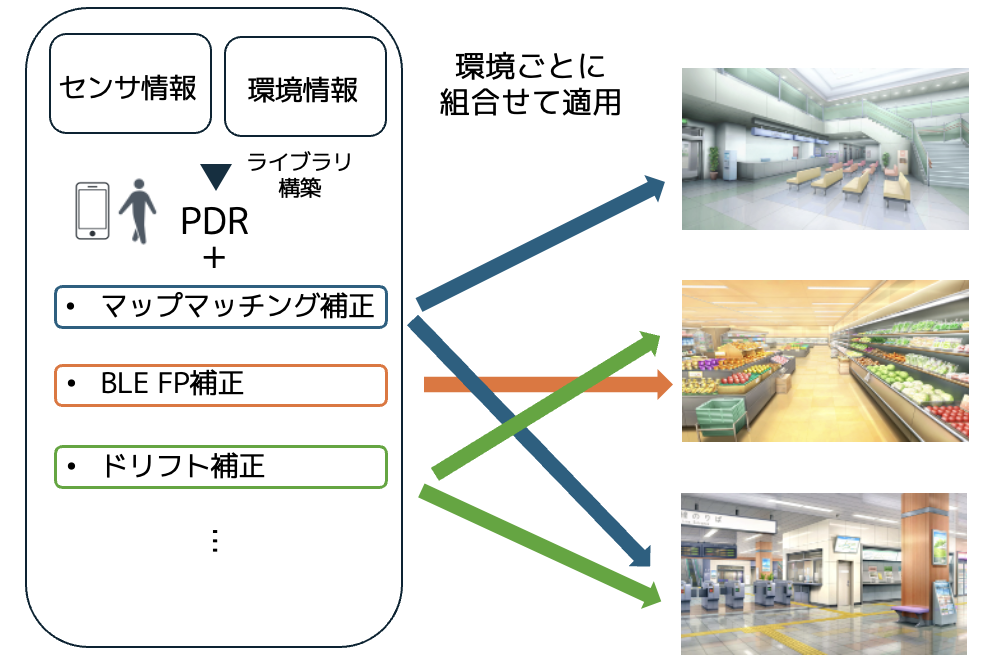
\includegraphics[width=80mm]{image/first.png}
	\caption{様々な状況と環境に対応できる\\PDRベースの
		屋内位置推定ライブラリの概要}    \label{fig:overview}
\end{figure}



\section{関連研究}
絶対位置推定に関する研究がある.
これは特定の基準点からの情報を元に位置を推定する手法である.
例えばBluetoothやWi-Fiなどの電波を利用した推定手法がある.
これらの電波を利用した推定手法はTriangulation方式,Fingerprint(以下,FP)方式,Proximity方式の3つに分類される
\cite{wireless-lan-summary}.
Triangulation方式を使用した研究として屋内に設置した近接特化型のBLEビーコン3つからの電波強度を
利用して三角測量を行い位置推定を行う研究がある\cite{ble-indoor}\cite{ble-tandem}\cite{triangulation-kalman}.
FP方式は特定の地点でのAPからの電波強度モデルを作成して,
実際の測定値をこのモデルの情報と照合して位置を推定する方式である.
この方式はデータ収集コストが大きい点やモデルを作成しても
環境の変化によってモデルの信頼性が低下してしまう問題があり,
それらの問題への対策を行った様々な研究がある
\cite{gaussian-mixture-model}
\cite{wireless-lan-cost-reduction}
\cite{fingerprint-auto-update}
\cite{wi-fi-fingerprint-domain}.
Promixity方式は特定のAPからの強い電波を受信した際,
そのAP付近にいると見なし推定する手法である.
これらの手法は状況に合わせて使いわけを行い組み合わせるとより精度の高い位置推定ができる.
Proximity方式とFP方式を併用した推定手法に関する研究がある\cite{proximity-fingerprint}.
この研究ではWi-FiのFP方式で位置を推定する前に有用に推定できるAPの絞りこみを行っている.
電波以外推定手法として磁気データを使用して位置推定を行う研究\cite{pdr-mag}や,
赤外線を使用して位置推定を行う研究\cite{infrared},カメラを利用した研究\cite{camera}などがある.

PDRと絶対位置推定を組み合わせて屋内位置推定を行う研究がある.
PDRは手法の性質上ある地点からの相対的な位置を推定する手法であるため,
位置推定をするには絶対位置推定と組み合わせる必要がある.
またPDRには1章で述べた誤差が蓄積する問題も存在する.
PDRとWi-Fiの受信強度を用いたProximityの位置推定を行う研究\cite{pdr-wifi}がある.
この研究では加速度センサ,地磁気センサ,気圧センサの値を用いて既知地点からの位置推定を行う.
Wi-Fi APからの電波受信強度が特定の閾値を越えている場合はProximityの位置推定に切り替える.
これによってPDRで生じる誤差の補正を行っている.
BLEビーコンの受信信号強度の変異を利用した移動変異推定とPDRとの併用による累積測位誤差の補正を行う研究\cite{pdr-ble}がある.
この手法ではWi-FiのAPからの情報を使うのでなくBLEビーコンを配置してその電波と位置情報をもとにPDRの誤差の補正を行っている.
またPDRとマップマッチングを組み合わせて位置推定を行う研究\cite{pdr-map}がある.
この手法ではマップマッチングを用いて歩幅を動的に更新を行い誤差を低減したPDR手法を提案している.
これらの研究で示されているようにPDRと絶対位置測位を組み合わせた手法は,
お互いのデメリットを補えるため屋内位置推定をする上で有用な手法である.

本研究でもPDRによる位置推定を行い,その結果に対してBLEビーコンの電波強度を使用した補正やマップマッチングによる
補正をなどが行えるライブラリを検討する.
さらに初期位置や終了位置の有無などの様々な状況の情報で補正できるようなライブラリの検討を目指す.


\subsection{ライブラリ}
\begin{table*}[ht]
	\centering
	\scalebox{0.7}{
		\begin{tabular}{|c|c|c|c|c|c|c|c|c|c|c|c|c|c|} % Change 'l' to 'c' for center alignment
			\hline
			              & 関数名                                                    & \multicolumn{4}{c|}{センサ情報}   & \multicolumn{4}{c|}{環境情報}    & \multicolumn{4}{c|}{その他}                                                                                                                                                                                                                                                                                                                             \\ \hline
			              &                                                        &                              &                              &                              & \multicolumn{1}{c|}{BLEビーコン} &                              & \makecell{磁気                                                                                                } & \multicolumn{2}{c|}{BLEビーコン} & \multicolumn{2}{c|}{正解初期}    & \multicolumn{2}{c|}{正解補正}                                                 \\ \cline{6-6} \cline{8-8} \cline{9-9} \cline{10-10}\cline{11-12}\cline{13-14}
			              &                                                        & 加速度                          & 角速度                          & 角度                           & 電波強度                         & フロアマップ                       & FP                                                                                                            & 基地局位置                        & FP                           & 座標                               & 方向 & 座標                           & 方向 \\ \hline
			基本PDR         & estimate\_trajectory                                   & \multicolumn{1}{c|}{$\circ$} & \multicolumn{1}{c|}{$\circ$} &                              &                              &                              &                                                                                                               &                              &                              & \multicolumn{1}{c|}{$\triangle$} &    &                              &    \\ \hline
			角速度から角度推定     & convert\_to\_angle\_from\_gyro                         &                              & \multicolumn{1}{c|}{$\circ$} &                              &                              &                              &                                                                                                               &                              &                              &                                  &    &                              &    \\ \hline
			ドリフト補正        & remove\_drift\_in\_angle                               & \multicolumn{1}{c|}{$\circ$} &                              & \multicolumn{1}{c|}{$\circ$} &                              &                              &                                                                                                               &                              &                              & \multicolumn{1}{c|}{$\circ$}     &    & \multicolumn{1}{c|}{$\circ$} &    \\ \hline
			初期方向補正 フロアマップ & rotate\_trajectory\_to\_optimal\_alignment\_using\_map & \multicolumn{1}{c|}{$\circ$} &                              & \multicolumn{1}{c|}{$\circ$} &                              & \multicolumn{1}{c|}{$\circ$} &                                                                                                               &                              &                              & \multicolumn{1}{c|}{$\triangle$} &    &                              &    \\ \hline
			初期方向補正 BLE    & rotate\_trajectory\_to\_optimal\_alignment\_using\_ble & \multicolumn{1}{c|}{$\circ$} & \multicolumn{1}{c|}{$\circ$} &                              & \multicolumn{1}{c|}{$\circ$} &                              &                                                                                                               & \multicolumn{1}{c|}{$\circ$} &                              & \multicolumn{1}{c|}{$\triangle$} &    &                              &    \\ \hline
			マップマッチング補正    & move\_unwalkable\_points\_to\_walkable                 & \multicolumn{1}{c|}{$\circ$} & \multicolumn{1}{c|}{$\circ$} &                              &                              & \multicolumn{1}{c|}{$\circ$} &                                                                                                               &                              &                              &                                  &    &                              &    \\ \hline
			安定歩行区間補正      &                                                        & \multicolumn{1}{c|}{$\circ$} & \multicolumn{1}{c|}{$\circ$} &                              &                              &                              &                                                                                                               &                              &                              &                                  &    &                              &    \\ \hline
			初期方向補正 BLE FP &                                                        & \multicolumn{1}{c|}{$\circ$} & \multicolumn{1}{c|}{$\circ$} &                              &                              &                              &                                                                                                               &                              & \multicolumn{1}{c|}{$\circ$} &                                  &    &                              &    \\ \hline
		\end{tabular}
	}
	\caption{関数に必要な情報とその対応表} \label{}
	\textit{注: $\circ$は必須引数,$\triangle$はオプショナル引数を示す} \label{tab:my_label}
\end{table*}


関数に必要な引数の情報とその対応表を表1に示す.
詳しい関数の説明や内部実装については後述する.
引数の情報は大きく分けてセンサ情報,環境情報,その他の3つに分けられる.
センサ情報はスマートフォンから得られる加速度,角速度,磁気センサ,BLEビーコンの電波情報などが含まれる.
環境情報はフロアマップ情報,フロアマップにおける各BLEビーコンの配置情報などが含まれる.
これらの環境情報は全てセンサデータが与えられる前に得られる情報である.
その他はセンシング中,またはセンシング前に得られる情報であり,初期位置,終了位置などの情報が該当する.


\begin{table}[h]
	\centering
	\begin{tabular}{lll}
		\toprule
		カラム名 & 単位        & データ型  \\
		\midrule
		ts   & s (秒)     & float \\
		x    & m/s\(^2\) & float \\
		y    & m/s\(^2\) & float \\
		z    & m/s\(^2\) & float \\
		\bottomrule
	\end{tabular}
	\caption{加速度 DF}
\end{table}

\begin{table}[h]
	\centering
	\begin{tabular}{lll}
		\toprule
		カラム名 & 単位             & データ型  \\
		\midrule
		ts   & s (秒)          & float \\
		x    & rad/s (ラジアン/秒) & float \\
		y    & rad/s (ラジアン/秒) & float \\
		z    & rad/s (ラジアン/秒) & float \\
		\bottomrule
	\end{tabular}
	\caption{角速度 DF}
\end{table}


\begin{table}[ht]
	\centering
	\label{tab:first-coord-dict}
	\begin{tabular}{lll}
		\hline
		      & {データ型}         & {説明}          \\ \hline
		key   & \texttt{str}   & xまたはy         \\ \hline
		value & \texttt{float} & \makecell{座標} \\ \hline
	\end{tabular}
	\caption{正解初期座標 DICT}
\end{table}




\begin{table}[h]
	\centering
	\begin{tabular}{lll}
		\toprule
		カラム名 & 単位      & データ型  \\
		\midrule
		ts   & s (秒)   & float \\
		x    & m(メートル) & float \\
		y    & m(メートル) & float \\
		\bottomrule
	\end{tabular}
	\caption{座標DF}
\end{table}


\begin{table}[h]
	\centering
	\begin{tabular}{lll}
		\toprule
		カラム名 & 単位         & データ型  \\
		\midrule
		ts   & s (秒)      & float \\
		x    & rad (ラジアン) & float \\
		y    & rad (ラジアン) & float \\
		z    & rad (ラジアン) & float \\
		\bottomrule
	\end{tabular}
	\caption{角度 DF}
\end{table}




説明する関数の引数に必要な情報は全て表1と紐づいている.
言語にはPythonを使用した.Pythonはデータ解析や機械学習などの分野で広く使われており,
ライブラリを使用するユーザーにとっても比較的扱いやすい利点がある.
まず基本的なPDRの処理を行う関数をListing\ref{lst:pdr-trajectory}に示す.
この関数では加速度データフレーム(以下,DF),角速度DFを使用して位置推定を行う.
加速度DF,角速度DFのデータフレームのカラム名とデータ型を表2,表3に示す.
オプショナル引数として正解初期座標(ground\_truth\_first\_point)を与えられる.
正解初期座標は辞書型で表4に示す.
戻り値は時間経過に伴う2次元座標のDFと角度のDFであり,それぞれのカラム名とデータ型を表5,表6に示す.
戻り値で角度DFを返す理由として,次の補正処理をする際に角速度よりも扱いやすいためである.

歩幅の推定を行っている研究は多くある.
機会学習を用いた研究\cite{stride-length-auto-learning},
多変量解析を用いた研究\cite{stride-length-multi},
超音波センサーガジェットを用いた研究\cite{stride-length-ultrasonic}などがある.
本関数の内部処理では歩幅の値は固定値として扱っている.
本来であれば歩幅は身長,性別,年齢などの複数の要素によって動的に変化するため
固定値なのはありえず,先ほど挙げた研究のように歩幅を推定する必要がある.
しかし本ライブラリの目的は正確な歩幅を用いたPDRによる位置推定ではない.
PDRで推定した歩行軌跡を環境情報などを用いて補正を行い軌跡全体の最適化を行えるライブラリの検討である.
そのため歩幅の推定は行わず固定値として扱う.
また同様の理由で歩行タイミングの検出も正確には行わず,加速度の値が特定の閾値を超えた時に
歩行タイミングとして扱っている.
図\ref{fig:pdr}にリスト\ref{lst:pdr-trajectory}を用いてPDRによる位置推定を行った結果を示す.
LiDARで取得した座標をもとに出力された軌跡を図\ref{fig:gt-trajectory}に示す.
これを本論では正解軌跡とする.
図\ref{fig:pdr}と図\ref*{fig:gt-trajectory}を比較するとPDRによる軌跡は正解軌跡と比べて大きくずれているのがわかる.
PDR特有の解決すべきものとして
軌跡そのものの形状を正解奇跡に近づける問題と絶対位置との関連付けの問題がある.
本ライブラリを用いてこれらの問題を解消し正解軌跡に近づけていく.

% 文書内
\begin{lstlisting}[caption={基本PDR}, label=lst:pdr-trajectory]
Axis2D = Literal["x", "y"]
def estimate_trajectory(
    acc_df: pd.DataFrame,
    gyro_df: pd.DataFrame,
    *,
    ground_truth_first_point: dict[Axis2D, float] | None = None,
) -> tuple[pd.DataFrame, pd.DataFrame]:
\end{lstlisting}

\begin{figure}[h]
	\centering
	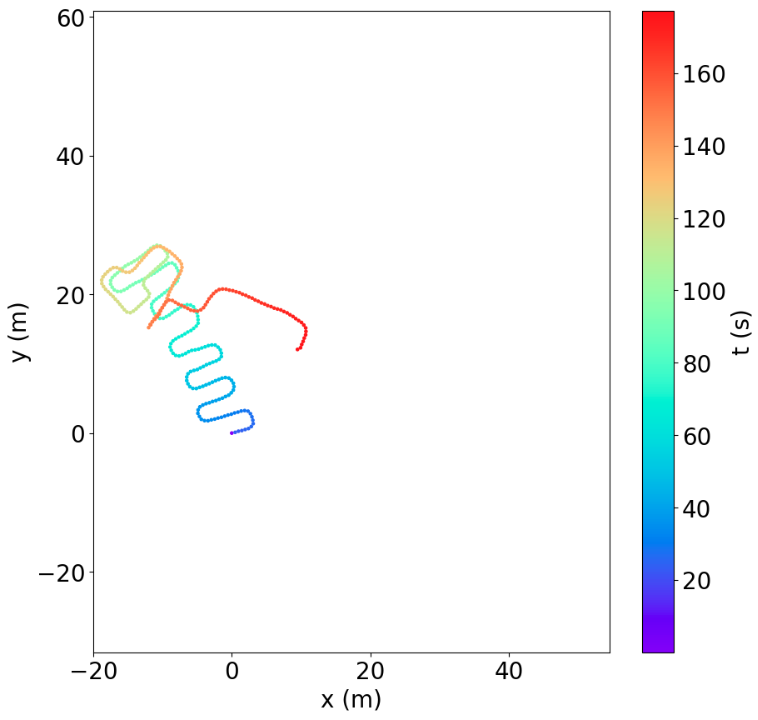
\includegraphics[width=80mm]{image/pdr.jpg}
	\caption{PDRによる軌跡}    \label{fig:pdr}
\end{figure}

Listing\ref{lst:pdr-trajectory}に示される関数に正解初期座標を
を与えたのが図\ref{fig:pdr-move}である.
予め正解座標が判明している場合はPDRによる軌跡の初期位置を補正できる.

\begin{figure}[h]
	\centering
	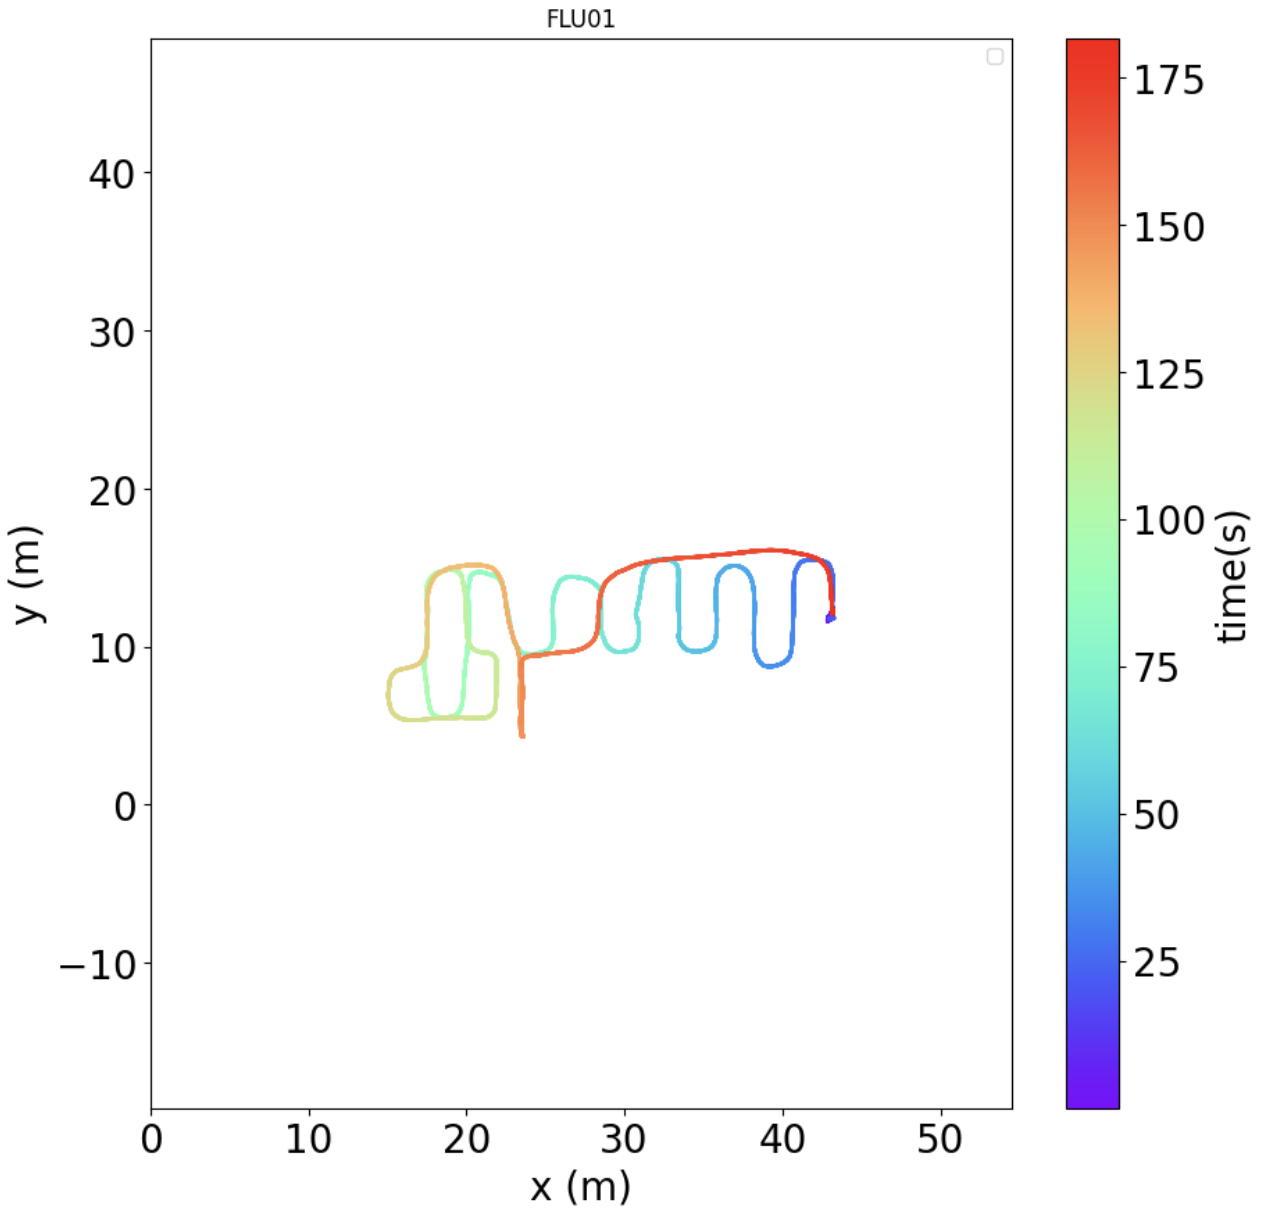
\includegraphics[width=80mm]{image/gt2.jpg}
	\caption{正解軌跡}    \label{fig:gt-trajectory}
\end{figure}

\begin{figure}[h]
	\centering
	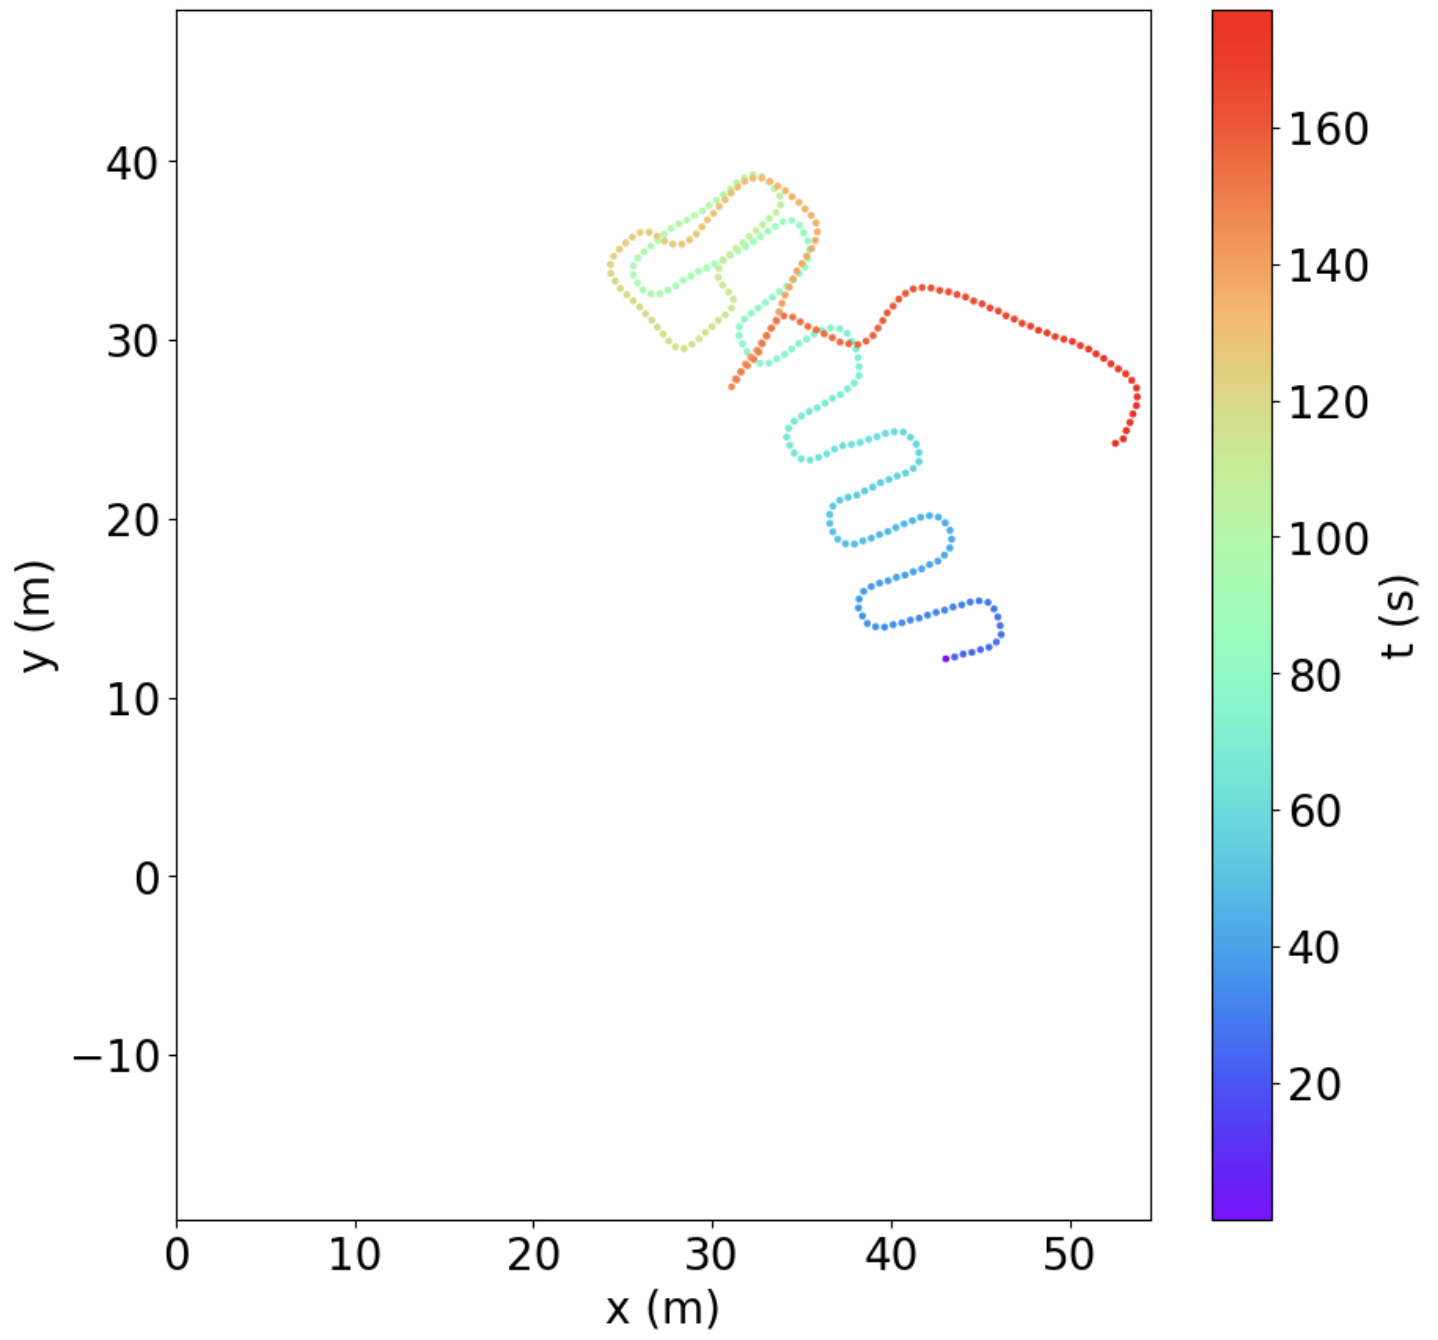
\includegraphics[width=80mm]{image/pdr-move.jpg}
	\caption{正解初期座標が存在}    \label{fig:pdr-move}
\end{figure}


図\ref{fig:pdr-move}の軌跡にはPDR特有のドリフト現象が見られる.
PDRでは角速度から進行方向を求めてその方向を元に歩行軌跡を描く.
そのため角速度センサーにわずかなでも誤差が含まれると時間経過とともにその誤差が大きくなり軌跡の形状が本来の軌跡から外れる.
この問題を解決するには角速度データに含まれる累積誤差を取り除く必要がある.


\begin{lstlisting}[caption={ドリフト除去}, label=lst:remove-drift]
def remove_drift_in_angle_df(
    acc_df: pd.DataFrame,
    angle_df: pd.DataFrame,
    ground_truth_point_df: pd.DataFrame,
) -> tuple[pd.DataFrame, pd.DataFrame]:
\end{lstlisting}

% このアルゴリズムは,角速度データに含まれる累積誤差を取り除くことで,PDRに基づく軌跡の精度を向上させる。
ドリフトを取り除く関数をListing\ref{lst:remove-drift}に示す.
引数として加速度DF,角速度DF,正解座標DFを受け取る
戻り値は時間経過に伴う2次元座標のDFと角度のDFを返す.
ドリフト補正のプロセスは,ドリフトの値を動的に計算し,それを各時刻の角度データから差し引く.
このドリフト補正プロセスは,式(1)で表される.
$\theta'(t)$は時間$t$における補正後の角度,$\theta(t)$は補正前の角度,
$\mathrm{d}$はドリフトの大きさを意味する.
この式は,時間経過に伴うドリフトの累積効果を補正するために使用される.

\vspace{5mm} % 5mmの空白を追加。必要に応じて値を調整してください。

\begin{equation}
	\theta'(t) = \theta(t) - (\mathrm{d} \times (t))
\end{equation}

\vspace{5mm} % 5mmの空白を追加。必要に応じて値を調整してください。

補正の効果を評価し適切なドリフトを見つけるために,ユークリッド距離を用いて,2つの正解座標の差異を計算する.
式(2)は,正解座標$(x_{\mathrm{n}}, y_{\mathrm{n}})$と正解座標$(x_{\mathrm{n+1}}, y_{\mathrm{n+1}})$との間のユークリッド距離$\mathrm{E}$を示している.
この式に基づきドリフト値に対してグリッドサーチを行い距離が最小になるドリフト値を探す.
最小のドリフト値を角度DFから引きそれに基づいた座標DFと角度DFを返す.
図\ref{fig:pdr-remove-drift}に示すように,ドリフト補正後の軌跡は,元の軌跡と比較して正解軌跡の形状に近づいている.
このアルゴリズムでは正解座標$(x_{\mathrm{n}}, y_{\mathrm{n}})$と正解座標$(x_{\mathrm{n+1}}, y_{\mathrm{n+1}})$の距離が近い時に特に有効である.
この処理は$(x_{\mathrm{n+2}}, y_{\mathrm{n+2}})$など2つ以上の座標が存在する場合も同様に適用できる.

\vspace{5mm} % 5mmの空白を追加。必要に応じて値を調整してください。
\begin{equation}
	\mathrm{E} = \sqrt{(x_{\mathrm{g}} - x_{\mathrm{ref}})^2 + (y_{\mathrm{g}} - y_{\mathrm{ref}})^2}
\end{equation}
\vspace{5mm} % 5mmの空白を追加。必要に応じて値を調整してください。

\begin{figure}[h]
	\centering
	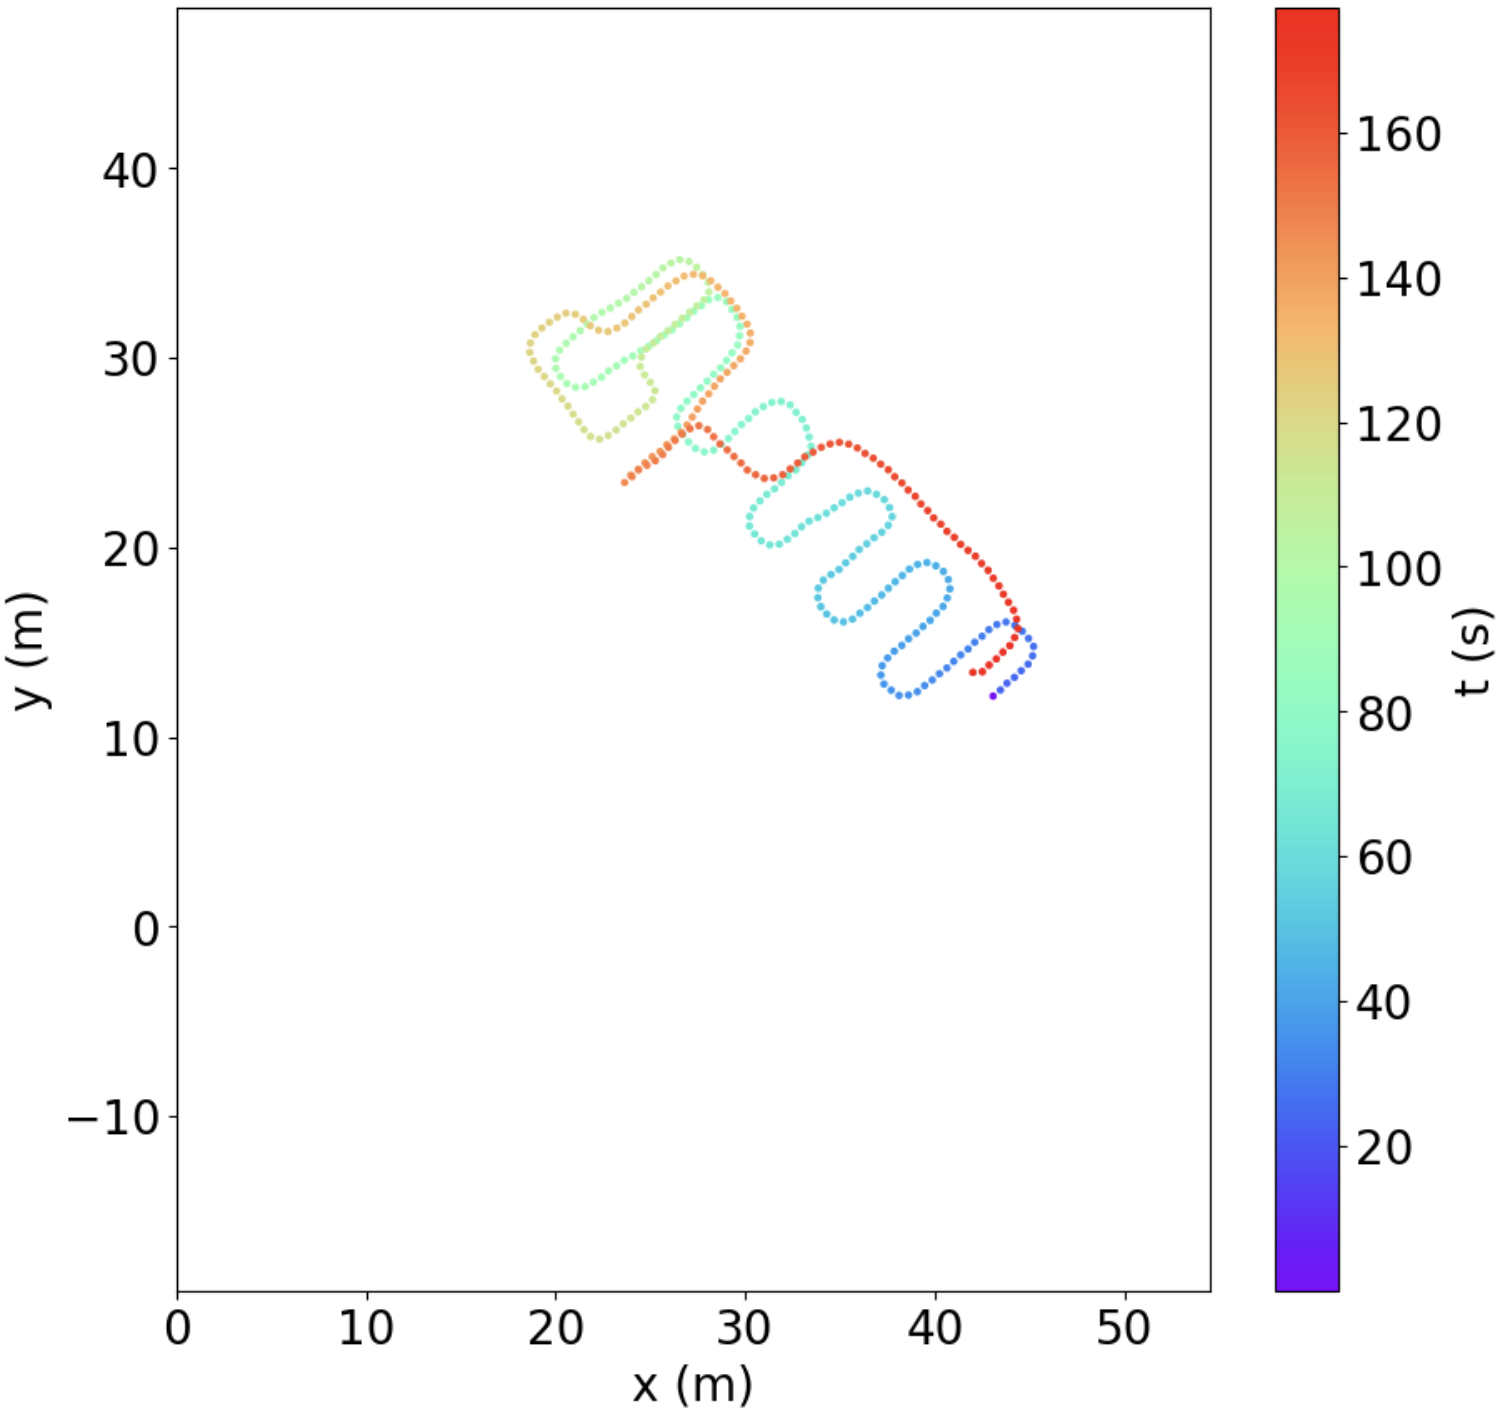
\includegraphics[width=80mm]{image/pdr-remove-drift-two.jpg}
	\caption{ドリフト補正後の軌跡}    \label{fig:pdr-remove-drift}
\end{figure}


図\ref{fig:pdr-remove-drift}の軌跡の問題点として初期方向の誤差がある.
初期方向が誤っていると,歩行者の実際の移動経路と大きく異なる軌跡になる.
この問題を解決するためには,適切な初期方向を見つけて軌跡全体を回転させる必要がある.
フロアマップ情報を元に軌跡を回転させる関数をListing\ref{lst:pdr-rotate}に示す.
引数として加速度DF,角度DF,表\ref{tab:map_dict}に示すフロアマップ情報DICT,フロア名,及びマップの1pxあたりの距離を受け取る.
内部の処理としては軌跡を回転させその時の水平垂直方向の割合を計算する.
軌跡における垂直成分と水平成分を可視化したものが図\ref{fig:color}である.
この割合が最も大きい回転角度をグリッドサーチを用いて探し最適な角度を見つける.
しかしこの処理だけでは適切な初期方向は絞り込めない.
割合が大きいものがあっても90度回転させるごとに水平垂直方向の割合が同一になるため4つの角度から適切な初期方向を見つける必要がある.
この絞り込みの処理としてマップ上の通行可能,不可能な座標の情報を利用する.
各回転角度での軌跡座標がマップ上で通行可能なポイントの数を計算し最も多いポイントを持つ回転角度を選択する.
この処理を適用した結果が図\ref{fig:pdr-rotate}である.
補正前と比べて軌跡の初期方向が正解軌跡に近づいている.

\begin{lstlisting}[caption={初期方向補正}, label=lst:pdr-rotate]
def rotate_trajectory_to
		_optimal_alignment_using_map(
    acc_df: pd.DataFrame,
    angle_df: pd.DataFrame,
    map_dict: dict[str, np.ndarray],
    floor_name: str,
    dx: float,
    dy: float,
    *,
    ground_truth_first_point: dict[Axis2D, float] | None = None,
) -> tuple[pd.DataFrame, pd.DataFrame]:
\end{lstlisting}

\begin{table}[ht]
	\centering
	\begin{tabular}{lll}
		\hline
		      & \textbf{データ型}       & \textbf{説明}             \\ \hline
		key   & \texttt{str}        & floorの名前                \\ \hline
		value & \texttt{np.ndarray} & \makecell{フロアマップの画像データ. \\各フロアのブール値の\\NumPy配列} \\ \hline
	\end{tabular}
	\caption{フロマップ DICT}
	\label{tab:map_dict}
\end{table}

\begin{figure}[h]
	\centering
	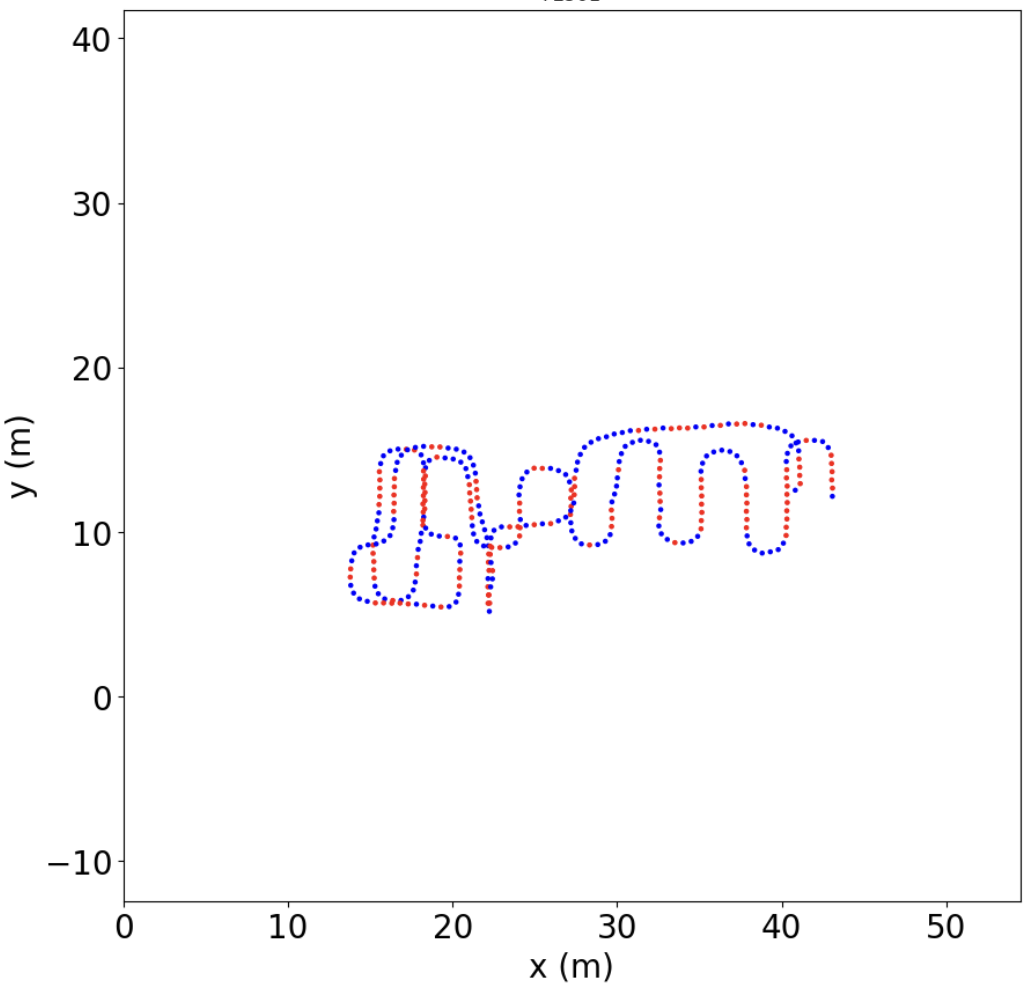
\includegraphics[width=80mm]{image/rb.jpg}
	\caption{垂直成分と水平成分の可視化}    \label{fig:color}
\end{figure}

\begin{figure}[h]
	\centering
	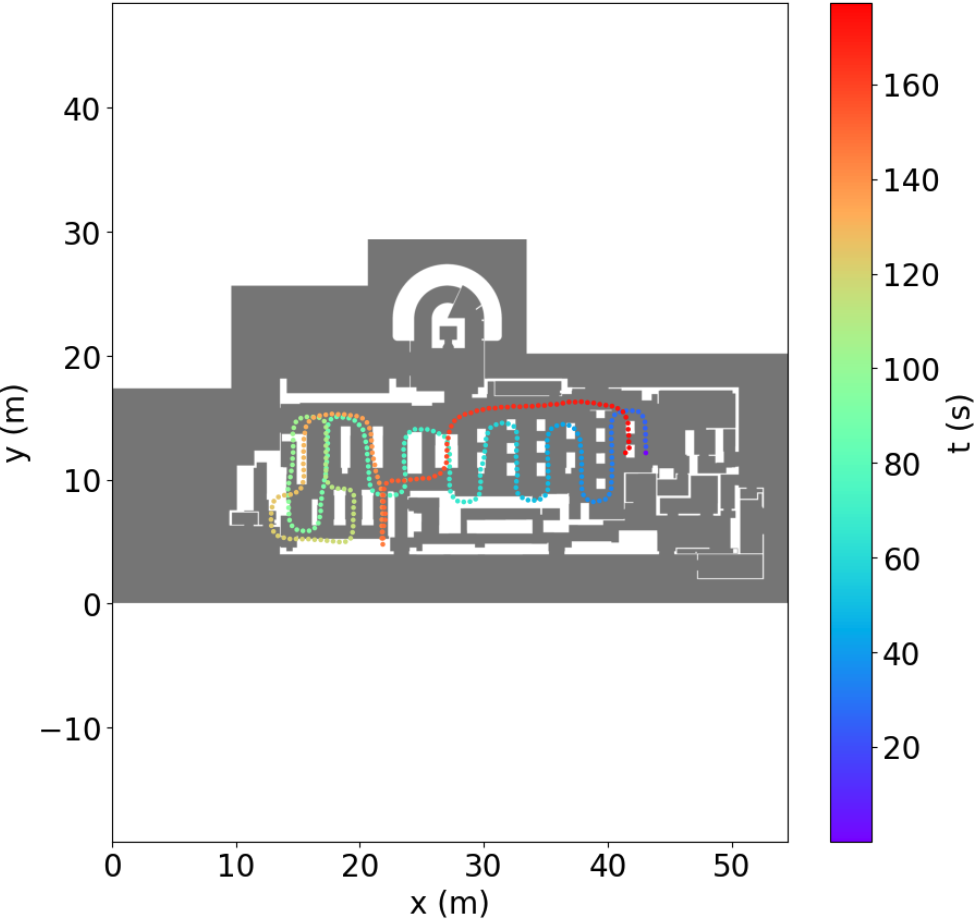
\includegraphics[width=80mm]{image/pdr-rotate.jpg}
	\caption{初期方向の補正後の軌跡}    \label{fig:pdr-rotate}
\end{figure}

フロアマップ情報を用いた初期方向補正ではマップの存在可能な点の分布によっては正しく機能しない場合がある.
別の方法としてBLEビーコンの情報を用いた初期方向補正を行う関数を提供する.
関数をListing\ref{lst:rotate-trajectory-using-ble}に示す.
この関数では加速度DF,角度DF,BLEビーコンの電波強度DF, BLEビーコンの基地局DFを受け取る.
BLEビーコンの電波強度DFとBLEビーコンの基地局DFのカラム名とデータ型を表6,表7に示す.
戻り値は時間経過に伴う2次元座標のDFと角度のDFを返す.
一定の強いRSSIの電波を受信した際の時間情報を元に時間的に近い推定軌跡の座標を取得する.
図\ref{fig:ble-merge}に示した図は時間的に近い推定軌跡の座標を時間経過に応じた色で表しており
青色の座標が配置されたBLEビーコンの座標を表している.

推定した軌跡の受信したBLEビーコンの基地局の座標との距離を計算する.
この総和が最小となるような回転角度をグリッドサーチで探し最適な角度に補正を行う.
BLEビーコンの基地局の座標との距離を計算する.

\begin{lstlisting}[caption={BLEを使用した初期方向補正}, label=lst:rotate-trajectory-using-ble]
def rotate_trajectory_to_optimal
		_alignment_using_ble(
    acc_df: pd.DataFrame,
    angle_df: pd.DataFrame,
    ble_scans_df: pd.DataFrame,
    ble_position_df: pd.DataFrame,
    *,
    ground_truth_first_point: dict[Axis2D, float] | None = None,
) -> tuple[pd.DataFrame, pd.DataFrame]:
\end{lstlisting}

\begin{figure}[h]
	\centering
	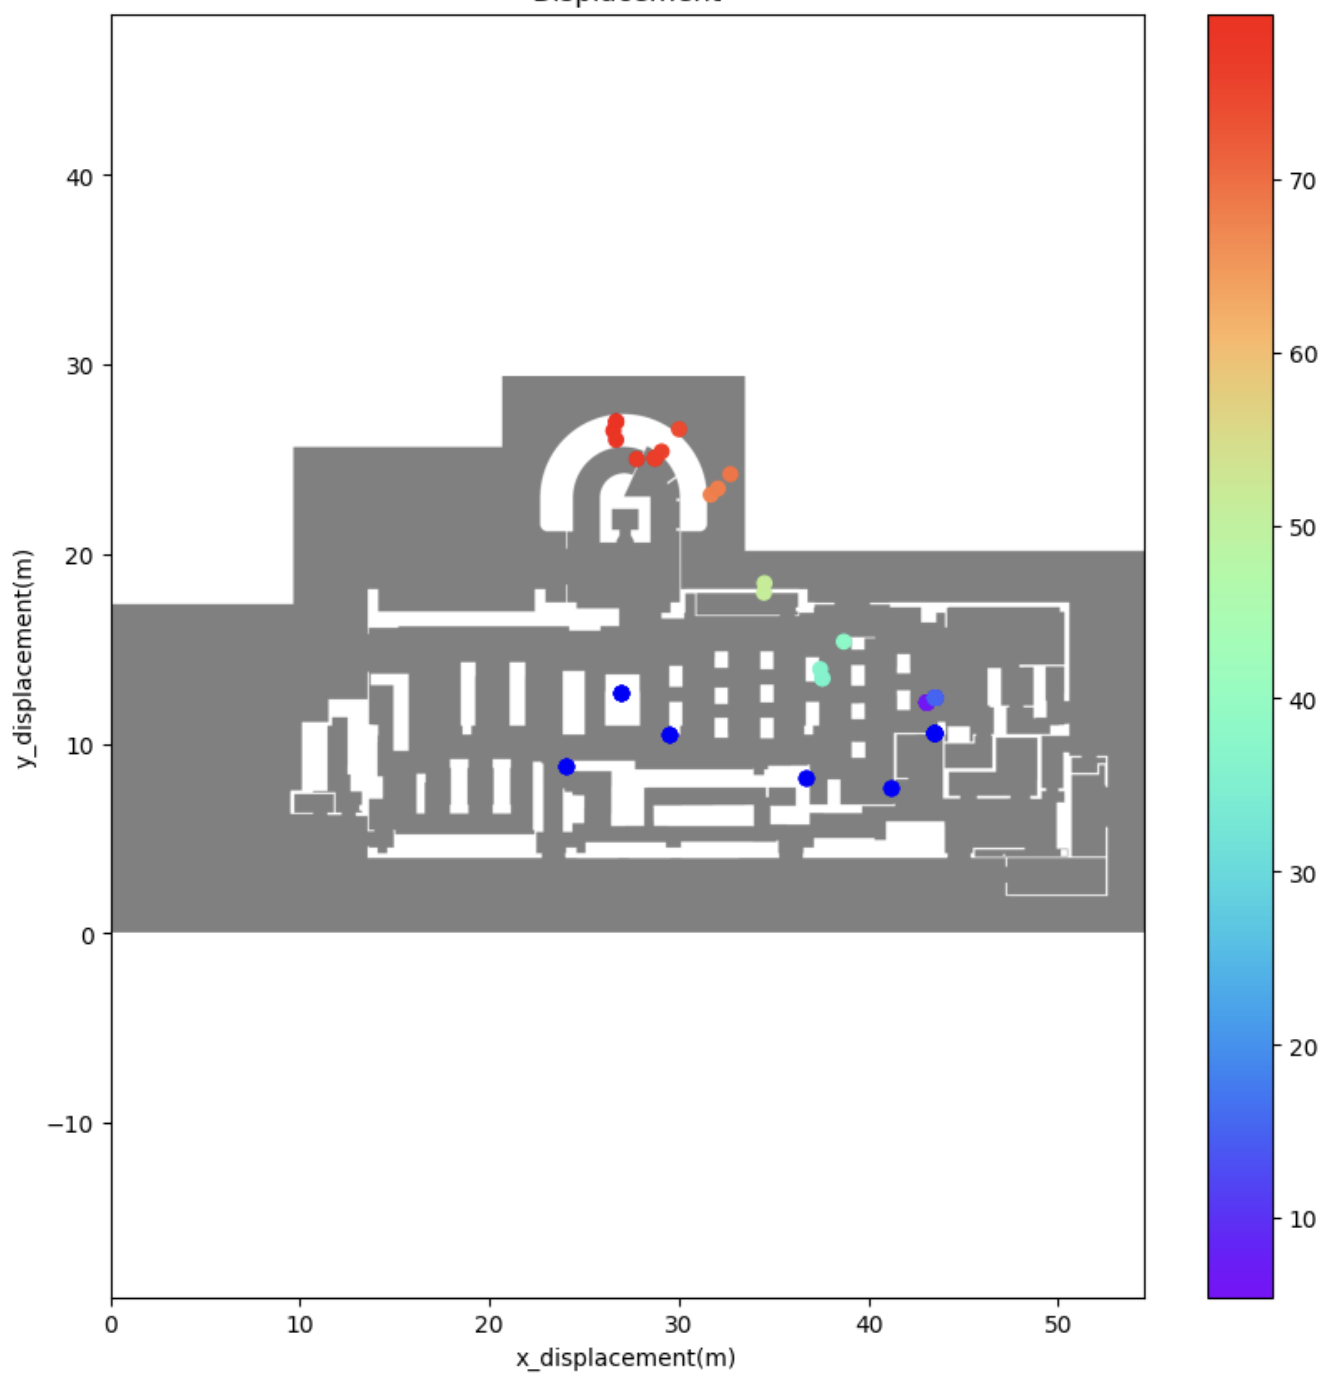
\includegraphics[width=80mm]{image/ble-merge.jpg}
	\caption{強いビーコン電波を受信した際の\\時間的に近い軌跡の座標}    \label{fig:ble-merge}
\end{figure}

\begin{table}[h]
	\centering
	\begin{tabular}{lll}
		\toprule
		カラム名      & 単位    & データ型  \\
		\midrule
		ts        & s (秒) & float \\
		bdaddress & なし    & str   \\
		rssi      & dBm   & int   \\
		\bottomrule
	\end{tabular}
	\caption{BLEビーコン電波強度DF}
\end{table}

\ref{fig:pdr-rotate}に示す軌跡の問題点として人間が歩行不可能領域を通過している点がある.
現実の人間がこのような場所を通過しないため,このような軌跡は不適切である.
そのため軌跡が歩行不可領域に存在する場合は,歩行可能な領域に移動させる処理が必要である.
この問題を解決する処理としてListing\ref{lst:map-matching}に示すマップマッチング補正関数を提供する.
マップマッチング補正関数は加速度DF,角度DF,フロアマップ情報DICT,フロア名,及びマップの1pxあたりの距離を受け取る必要がある.
戻り値は時間経過に伴う2次元座標のDFのみを返す.内部の処理の関係上補正後の角度DFは返すのが難しいためである.
関数内部ではまず加速度と角度のデータを基にして軌跡を推定する.
この軌跡に対して,各地点での座標が与えられたフロアマップ上の歩行可能な領域に存在するかどうかを検証する.
検証の結果,各地点での座標が歩行不可能な領域に存在する場合,当該座標から最も近い歩行可能な座標を幅優先探索アルゴリズムを
用いて探す.
該当する座標が見つかった場合,該当座標と該当座標以降の軌跡の座標を歩行可能な座標に平行移動して補正を行う.
当該座標の補正が終了後,次の座標に対して同様の処理を行う処理を繰り返す.
これによって軌跡の各地点が歩行可能な領域に存在するようになり,軌跡全体が最適化される.
図\ref{fig:map-matching}に示すように,マップマッチング補正後の軌跡では
歩行不可能な領域に存在していた地点がが歩行可能な地点に移動されている.

\begin{lstlisting}[caption={マップマッチング補正}, label=lst:map-matching]
def move_unwalkable_points_to_walkable(
    acc_df: pd.DataFrame,
    angle_df: pd.DataFrame,
    map_dict: dict[str, np.ndarray],
    floor_name: str,
    dx: float,
    dy: float,
    *,
    ground_truth_first_point: dict[Axis2D, float] | None = None,
) -> pd.DataFrame:

\end{lstlisting}

\begin{figure}[h]
	\centering
	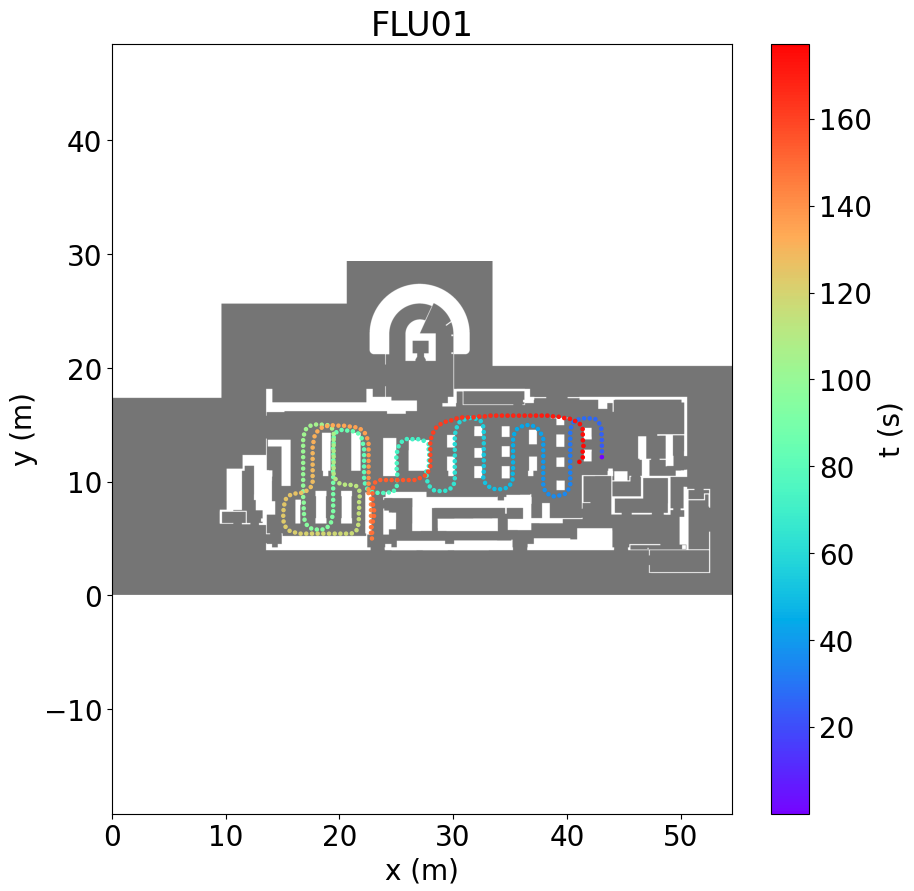
\includegraphics[width=80mm]{image/map-matching.png}
	\caption{マップマッチング補正後の軌跡}    \label{fig:map-matching}
\end{figure}


\begin{table}[h]
	\centering
	\begin{tabular}{lll}
		\toprule
		カラム名        & 単位 & データ型  \\
		\midrule
		bdaddress   & なし & str   \\
		x           & m  & float \\
		y           & m  & float \\
		floor\_name & なし & str   \\
		\bottomrule
	\end{tabular}
	\caption{BLEビーコン基地局 DF}
\end{table}


\section{ライブラリの検証と他環境における検討}
この章では提案したライブラリの有効性を検証する.
検証はxDR Challenge 2023での評価を基に行い,
また他環境でこれらのライブラリが適用可能かを検討する.

\subsection{xDR Challenge 2023環境での評価}


xDR Challenge 2023の環境についてあらためて詳細に説明する.
対象施設は高速道路のサービスエリアである.
対象の建物は2つあり,1つは2階建て,もう1つは平屋である.
提供される訓練データとスコアリングデータの詳細を表\ref{table:data}に示す.
BLEビーコンとしてMyBeacon(Aplix)\cite{beacon-aplix}を利用し,BLE信号は0.1秒ごとに発信される.
ビーコンの位置は,フロアマップの座標の (x, y, z) 位置として提供される.
競技に使用される9軸IMUセンサデータはAQUOS Sense 6(SHARP)により計測される.
正解のデータはハンドヘルド LiDAR (GeoSLAM ZEB-Horizon) を使用して約 100 Hz で測定される.
サンプリングデータは歩行時間が54秒から667秒までの全323個のデータが提供された.
スコアリングデータは歩行時間が134秒から234秒までの全9個データが提供された.
スコアリングはBLEビーコンのデータがないものとあるものでそれぞれ行われる.
9データのうち3個がBLEビーコンのデータが与えられず,残りの6個にはBLEビーコンのデータが与えられる.


\begin{table*}[ht]
	\centering
	\caption{提供データの概要}
	\scalebox{0.8}{
		\begin{tabular}{|l|l|l|l|l|}
			\hline
			データタイプ                        & 測定デバイス        & レート                                & 訓練データ & スコアリングデータ    \\ \hline
			加速度                           & AQUOS Sense 6 & 約100Hz                             & 使用可能  & 使用可能         \\ \hline
			角速度                           & AQUOS Sense 6 & 約100Hz                             & 使用可能  & 使用可能         \\ \hline
			磁気                            & AQUOS Sense 6 & 約100Hz                             & 使用可能  & 使用可能         \\ \hline
			BLE RSSI                      & AQUOS Sense 6 & 10Hzのビーコンから送信、AQUOS Sense 6で受信時に記録 & 使用可能  & 使用可能         \\ \hline
			正解位置 (Ground Truth) (x, y, z) & ZEB-Horizon   & 約100Hz                             & 使用可能  & 始めと終わりのみ使用可能 \\ \hline
			正解姿勢 (Ground Truth) (四元数)     & ZEB-Horizon   & 約100Hz                             & 使用可能  & 始めと終わりのみ使用可能 \\ \hline
			正解階層名 (Ground Truth)          & -             & 各パスの1階層名                           & 使用可能  & 使用可能         \\ \hline
		\end{tabular}
		ii		\label{table:data}
	}
\end{table*}

xDR Challenge 2023ではPDRベンチマーク標準化委員会によって
提供された評価フレームワークを使用して評価が行われた.
このフレームワークではl\_ce(CE:円形誤差),l\_ca(CA\_l:局所空間における円形精度),
l\_eag(誤差蓄積勾配),l\_ve(VE:速度誤差),l\_obstacle(障害物回避要件)
の5つの評価指標が用いられた.
総合評価指標は式\ref{eq:evaluation_index}に示す式で計算される.
このライブラリを使って得られた評価と各指標の重みを表\ref{table:evaluation_index}に示す.
l\_ce,l\_eag, l\_ve,l\_obstacleでは一定の精度を得られた.
しかしl\_caでは精度が低かった.
l\_caの値が低いと場合局所空間における位置推定誤差の分布が広い.
これは環境条件の変化やセンサデータの微妙な違いが,位置推定結果に大きな影響を与える可能性が高い.
この問題を解決するためには,PDRアルゴリズムを改善し,より精度の高い位置推定を行う必要がある.

\begin{equation}
	\begin{aligned}
		I_i = & W_{ce} \times I_{ce} + W_{ca} \times I_{ca}                                        \\
		      & + W_{eag} \times I_{eag} + W_{ve} \times I_{ve} + W_{obstacle} \times I_{obstacle}
	\end{aligned}
	\label{eq:evaluation_index}
\end{equation}


\begin{table}[ht]
	\caption{評価指数の概要}
	\centering
	\begin{tabular}{l|l|l}
		\hline
		指標                        & 値 (\%) & 重み   \\ \hline
		l\_ce(CE:円形誤差)            & 88.55  & 0.25 \\
		l\_ca(CA\_l:局所空間における円形精度) & 62.51  & 0.20 \\
		l\_eag(EAG:誤差蓄積勾配)        & 93.02  & 0.25 \\
		l\_ve(VE:速度誤差)            & 95.55  & 0.15 \\
		l\_obstacle(障害物回避要件)      & 93.48  & 0.15 \\
		l (総合評価指数)                & 86.25  &      \\ \hline
	\end{tabular}
	\label{table:evaluation_index}
\end{table}


\subsection{駅の構内での検討}
駅構内での位置推定をする場合を考える.
駅は多くの人々が日常的に使用する場所であり,駅を対象として位置推定の研究も行われるなど位置推定の需要が高い.
駅の改札は地上から続いてるものもあれば地下にあるものもある.
地下の場合は特に衛星からの電波が届きにくい場所であるためGPSが有効ではない.
このような環境ではPDRが有効な手法である.
駅の改札の位置は工事などがない限り,基本的に固定位置から変化しない.
改札を通った時の位置をPDRの正解初期座標として使用できる.
改札を通って出た後,乗り換えを行う場合がある.
このような場合は次の改札口を正解補正座標として利用できる.
ICなどを使って駅改札を通った場合,ユーザを一意に識別できる.
そのため特定のユーザが乗り換えをしたという情報を収集するのは比較的容易である.
正解初期地点と正解補正座標を利用すればListing\ref{lst:remove-drift}に示したドリフト補正を適用できる.
また全ての駅ではないがある一定規模以上の駅構内の場合フロアマップ情報が入手できる可能性が高い.
その場合フロアマップ情報を用いたListing\ref{lst:map-matching}のマップマッチング補正が適用できる.

\subsection{大学のキャンパスでの検討}
大学のキャンパスで位置推定をする場合を考える.
大学には屋外環境と屋内環境がある.
建物間の移動経路を把握する場合はGPSが有効である.
しかし大学の建物内での移動経路を把握する場合GPSでは困難である.
このような場合にPDRを軸とした移動経路の把握を検討できる.
大学は研究室やサ―クルなど異なるコミュニティが混在している.
それらは1つの組織が大本で管理しているのではなく個々が独立運営している.
このような場所でBLEビーコンを配置する場合,各コミュニティへの申請のコストや
,場合によっては配置を拒否される可能性がある.
BLEビ―コン以外の電波の利用を考えた場合,Wi-Fiの電波の利用が検討できる.
Wi-Fiの基地局なら基本的にどのコミュニティにも配置がしてあり,設置コストの面でBLEビーコンと比べると低い.
しかし既知のWi-Fiの基地局位置情報の把握はコストが大きい.
そのためこのような場所ではWi-Fiの電波を使ったFP補正が有効だと考えられる.
FPを使った手法なら基地局の位置情報を把握していない場合でも利用できる.
3章ではBLEビ―コンの元にFP処理を行う関数を実装した.
Wi-FiとBLEは通信範囲や消費電力などで異なる点はあり,
内部の処理や閾値を変化させる必要はあるが,基本的に与える引数やそのデ―タ形式を揃えれば同様に適用できる.
また部屋に出入りする際には固定の位置の出入り口がある.
個人がそこを出入りしたという情報を取得できれば,
正解初期座標や正解補正座標としてドリフト除去を適用できる.





\section{まとめ}
本論文では,環境情報などを利用したPDRベースの位置推定ライブラリの基礎検討を行った.
補正に利用できる情報をセンサ情報,環境情報,その他の3つに分類し,それぞれの情報を用いた補正処理を提案した.
その結果として,XDR Challenge 環境下では一定の精度を獲得した.
また他環境においても本ライブラリが適用可能であるか検討を行った.
課題としては,PDRアルゴリズムの改善や挙げられる.
また本論文は2次元の屋内位置推定のみを想定したライブラリ構成となっている.
現実の屋内では3次元に構成されるものが多いため,本ライブラリを3次元空間に適用できるような拡張を検討したい.
具体的にはスマートフォンの気圧センサの値を使用すれば相対的な階層間の移動の検知が可能である.
これとフロアマップ情報を組み合わせることで3次元空間での位置推定が実現できると考えられる.










\bibliography{dicomo}
\bibliographystyle{junsrt}

\end{document}
